%%%%%%%%%%%%%%%%%%%%%%%%%%%%%%%%%%%%%%%%%
%
% Optics and Radar -based observations
% Assignment 2
%
%%%%%%%%%%%%%%%%%%%%%%%%%%%%%%%%%%%%%%%%%

%----------------------------------------------------------------------------------------
%	DOCUMENT CONFIGURATIONS
%----------------------------------------------------------------------------------------
%   FINAL VERSION
\documentclass{article}

\title{\textbf {Optics and Radar Based Observations} \\ Assignment 2\\ Pulse Modulation Techniques} % Title

\def\authors{
Ivan \v Sinkarenko\\
Anuraj Rajendraprakash
}
\author{\authors}

\usepackage{graphicx}
\usepackage{fullpage}

% load package with ``framed'' and ``numbered'' option.
\usepackage[framed,numbered,autolinebreaks,useliterate]{mcode}

\begin{document}

\maketitle % Insert the title, author and date

\centerline{Referee: Dr. Anita Enmark}

%\vspace{10mm}
%\begin{figure}[h!]
%\centering
%\centerline{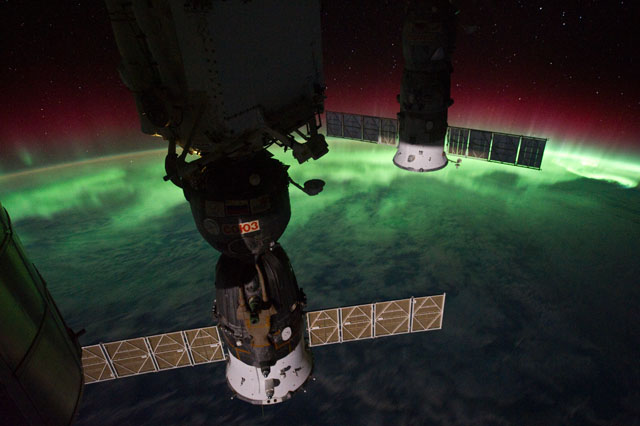
\includegraphics[width=\textwidth]{Figures/iss.jpg}}
%\label{fig:iss}
%\end{figure}

\setlength\parindent{0pt} % Removes all indentation from paragraphs

\renewcommand{\labelenumi}{\alph{enumi}.} % Make numbering in the enumerate environment by letter rather than number (e.g. section 6)
\clearpage

\tableofcontents

\listoffigures

\clearpage

%----------------------------------------------------------------------------------------
%	SECTION 1. Introduction
%----------------------------------------------------------------------------------------

\section{Introduction}
MST (mesosphere-stratosphere-troposphere) radars are applied to study winds, waves, turbulence and in- stability in the atmosphere. They usually operate near 50 MHz and also called VHF radars (VHF-very high frequency band between 30 MHz and 300 MHz).\\
\\
ESRAD (ESrange RADar) is VHF MST radar located in northern Sweden (6756N, 2104E). It has been in near continuous operation since June 1996. The purpose of the radar is to provide information on the dynamic state of the atmosphere - winds, waves, turbulence and layering from the troposphere up to the lower thermosphere (1 km -100 km altitude). ESRAD operates at a frequency of 52 MHz corresponding to a wavelength of 5.77 m. The transmitter consists of 72 1-kW solid-state modules that are grouped into 12 6-kW power blocks. The resulting peak power output power is 72 kW and the maximum duty cycle is 5\%. Pulse repetition frequency rates from 100 Hz to 16 kHz are possible. Pulse lengths correspond to height resolutions between 150 m and 3 km. The radar is capable of pulse coding the transmitted signals using both Barker and complementary codes. The radar has 6 separate receivers for detection of backscattered signals from the atmosphere. The complex (in-phase and quadrature) data samples are recorded using a 12-channel data acquisition unit. The bandwidth of the separate receiving elements is 2 MHz. Multiple receivers allows post-detection beam-steering and full spectral analysis of the returned signal. The digital processing system is able to process up to 256 heights per sample and integrates up to 4096 pulse repetitions per sample. The antenna consists of a 12 x 12 phased array of 5-element Yagis, each being approximately 6 m high. The Yagis are spaced about 4 m apart (corresponding to 0.7 times the radar wavelength). \cite{Enmark:2012a2}
 
%----------------------------------------------------------------------------------------
%	SECTION 2. Part 1
%----------------------------------------------------------------------------------------

\section{Part 1}

\begin{figure}[htb]
\begin{minipage}[t]{0.5\linewidth}
\centering
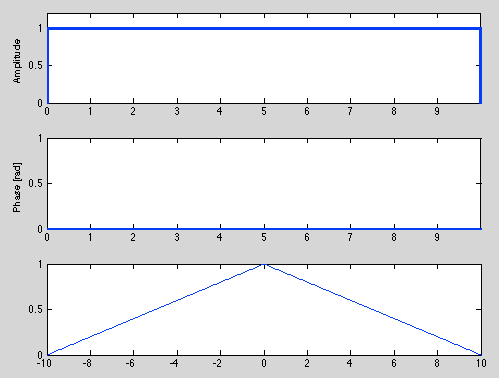
\includegraphics[width=8cm]{Figures/long_pulse_data.png}
\caption{Auto-correlation function of a long pulse.}
\label{fig:long_pulse_data}
\end{minipage}
%\hspace{0.5cm}
\begin{minipage}[t]{0.5\linewidth}
\centering
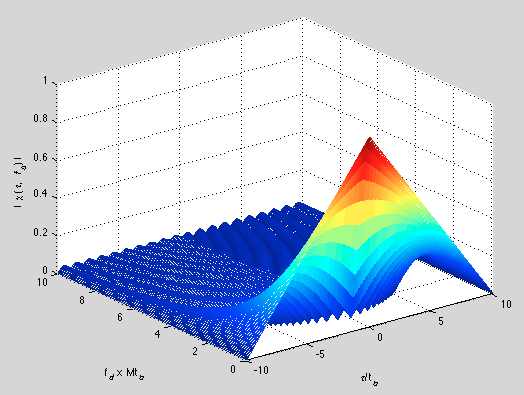
\includegraphics[width=8cm]{Figures/long_pulse_3d.png}
\caption{Ambiguity function of a long pulse.}
\label{fig:long_pulse_3d}
\end{minipage}
\end{figure}

\begin{figure}[htb]
\begin{minipage}[t]{0.5\linewidth}
\centering
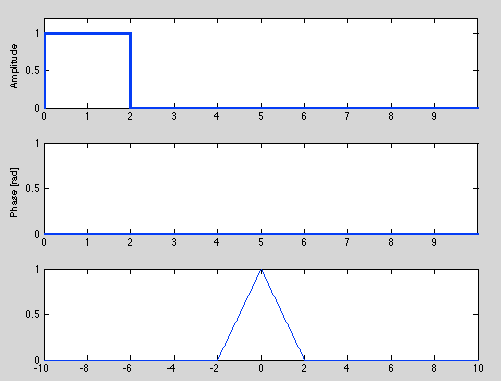
\includegraphics[width=8cm]{Figures/short_pulse_data.png}
\caption{Auto-correlation function of a short pulse.}
\label{fig:short_pulse_data}
\end{minipage}
%\hspace{0.5cm}
\begin{minipage}[t]{0.5\linewidth}
\centering
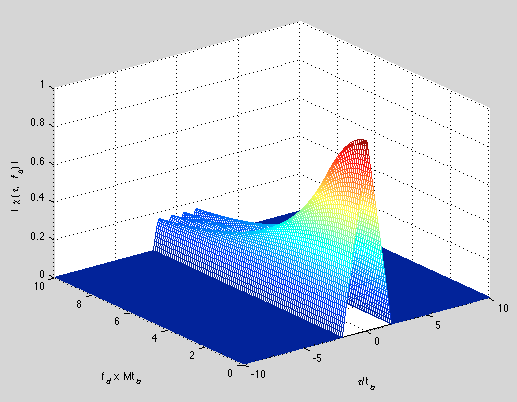
\includegraphics[width=8cm]{Figures/short_pulse_3d.png}
\caption{Ambiguity function of a short pulse.}
\label{fig:short_pulse_3d}
\end{minipage}
\end{figure}

\begin{figure}[htb]
\begin{minipage}[t]{0.5\linewidth}
\centering
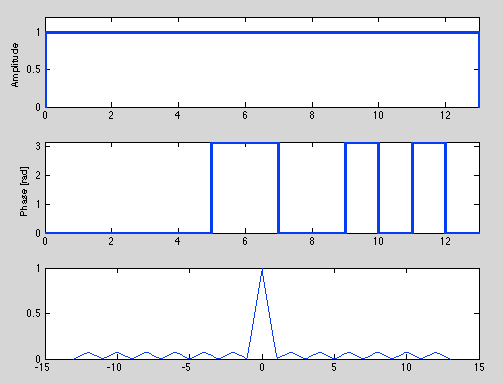
\includegraphics[width=8cm]{Figures/barker_data.png}
\caption{Auto-correlation function of Barker coding (13).}
\label{fig:barker_data}
\end{minipage}
%\hspace{0.5cm}
\begin{minipage}[t]{0.5\linewidth}
\centering
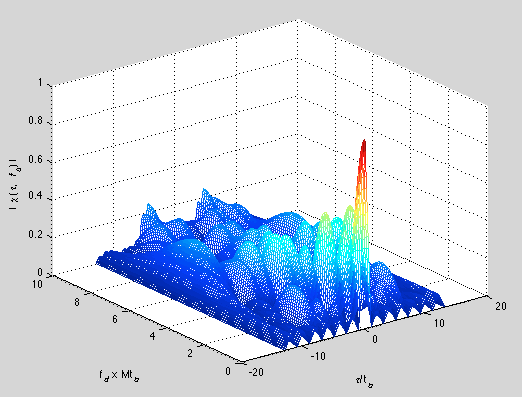
\includegraphics[width=8cm]{Figures/barker_3d.png}
\caption{Ambiguity function of Barker coding (13).}
\label{fig:barker_3d}
\end{minipage}
\end{figure}

\begin{figure}[htb]
\begin{minipage}[t]{0.5\linewidth}
\centering
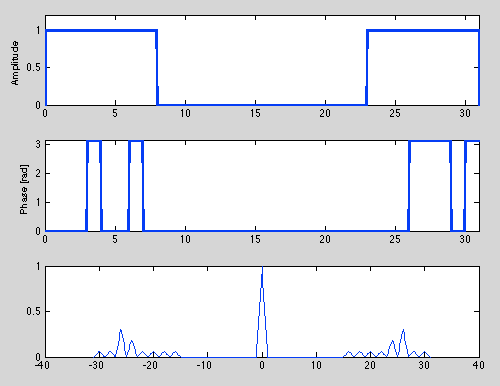
\includegraphics[width=8cm]{Figures/complementary_data.png}
\caption{Auto-correlation function of complementary coding (7).}
\label{fig:complementary_data}
\end{minipage}
%\hspace{0.5cm}
\begin{minipage}[t]{0.5\linewidth}
\centering
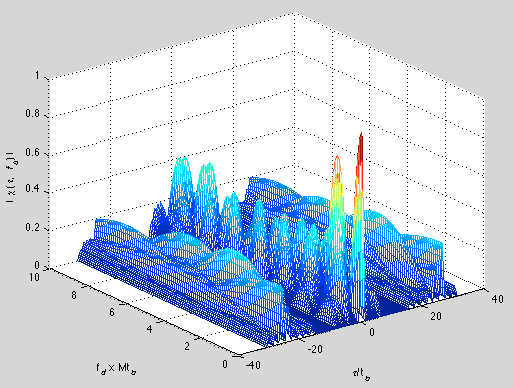
\includegraphics[width=8cm]{Figures/complementary_3d.png}
\caption{Ambiguity function of complementary coding (7).}
\label{fig:complementary_3d}
\end{minipage}
\end{figure}

\begin{figure}[htb]
\begin{minipage}[t]{0.5\linewidth}
\centering
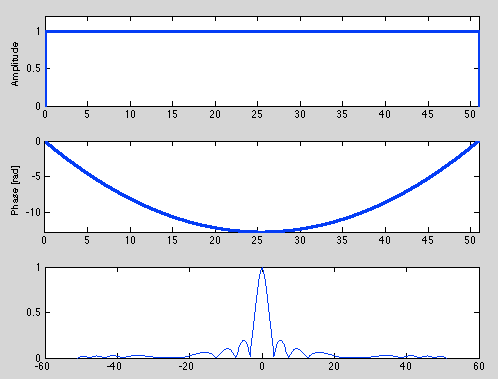
\includegraphics[width=8cm]{Figures/lfm_data.png}
\caption{Auto-correlation function of frequency coding with LFM.}
\label{fig:lfm_data}
\end{minipage}
%\hspace{0.5cm}
\begin{minipage}[t]{0.5\linewidth}
\centering
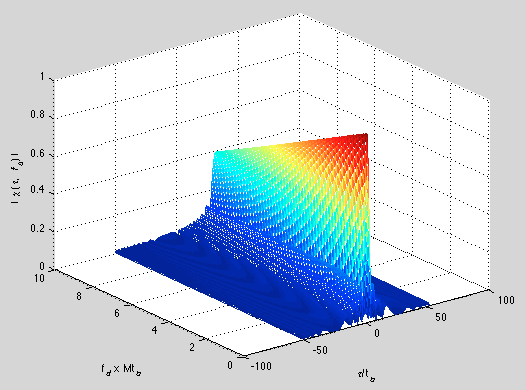
\includegraphics[width=8cm]{Figures/lfm_3d.png}
\caption{Ambiguity function of frequency coding with LFM.}
\label{fig:lfm_3d}
\end{minipage}
\end{figure}

%----------------------------------------------------------------------------------------
%	SECTION 3. Part 2
%----------------------------------------------------------------------------------------

\section{Part 2}

%----------------------------------------------------------------------------------------
%	SUBSECTION 3.1. Part 2A
%----------------------------------------------------------------------------------------

\subsection{Part 2A}

\begin{figure}[htb]
\begin{minipage}[t]{0.5\linewidth}
\centering
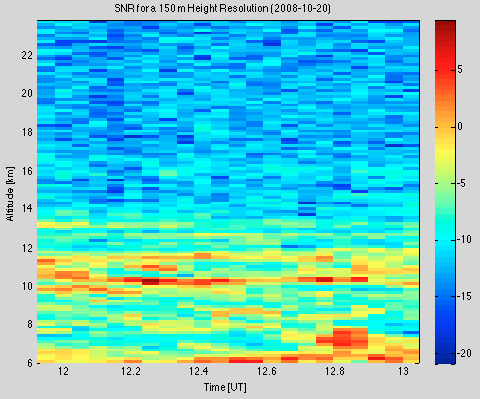
\includegraphics[width=8cm]{Figures/height_res_150m.png}
\caption{SNR data for 150 m height resolution.}
\label{fig:height_res_150m}
\end{minipage}
%\hspace{0.5cm}
\begin{minipage}[t]{0.5\linewidth}
\centering
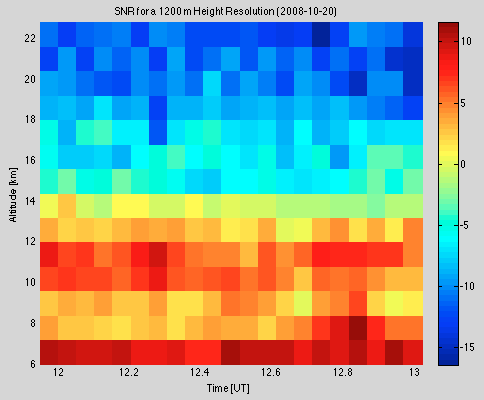
\includegraphics[width=8cm]{Figures/height_res_1200m.png}
\caption{SNR data for 1200 m height resolution.}
\label{fig:height_res_1200m}
\end{minipage}
\end{figure}

%----------------------------------------------------------------------------------------
%	SUBSECTION 3.2. Part 2B
%----------------------------------------------------------------------------------------

\subsection{Part 2B}

\begin{figure}[htb]
\begin{minipage}[t]{0.5\linewidth}
\centering
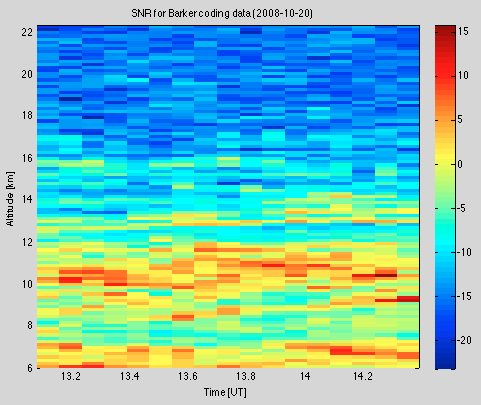
\includegraphics[width=8cm]{Figures/SNR_barker.png}
\caption{SNR for Barker coding data.}
\label{fig:SNR_barker}
\end{minipage}
%\hspace{0.5cm}
\begin{minipage}[t]{0.5\linewidth}
\centering
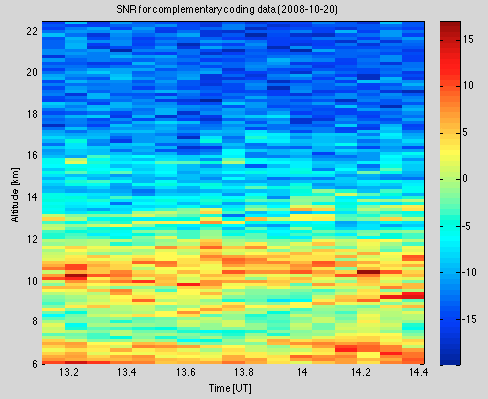
\includegraphics[width=8cm]{Figures/SNR_complementary.png}
\caption{SNR for complementary coding data.}
\label{fig:SNR_complementary}
\end{minipage}
\begin{minipage}[b]{0.5\linewidth}
\vspace{0.5cm}
\centering
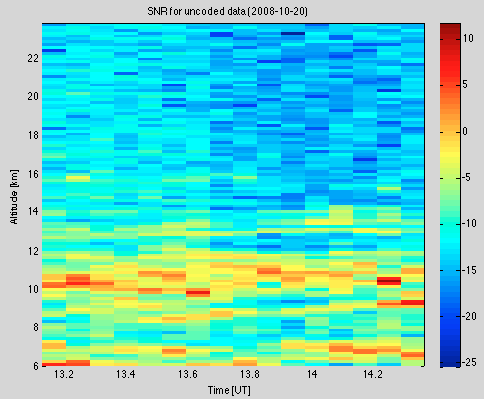
\includegraphics[width=8cm]{Figures/SNR_uncoded.png}
\caption{SNR for uncoded data.}
\label{fig:SNR_uncoded}
\end{minipage}
\end{figure}



\begin{figure}[htb]
\begin{minipage}[t]{0.5\linewidth}
\centering
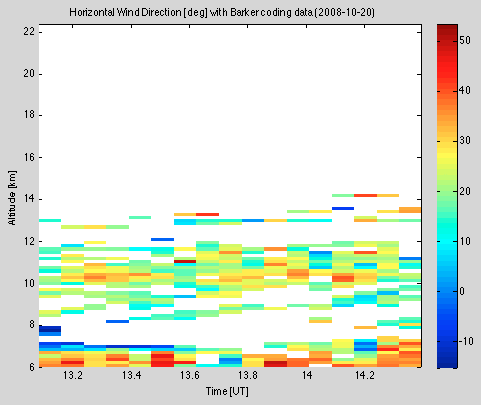
\includegraphics[width=8cm]{Figures/wind_dir_barker.png}
\caption{Horizontal wind direction with Barker coding data.}
\label{fig:wind_dir_barker}
\end{minipage}
\begin{minipage}[t]{0.5\linewidth}
\centering
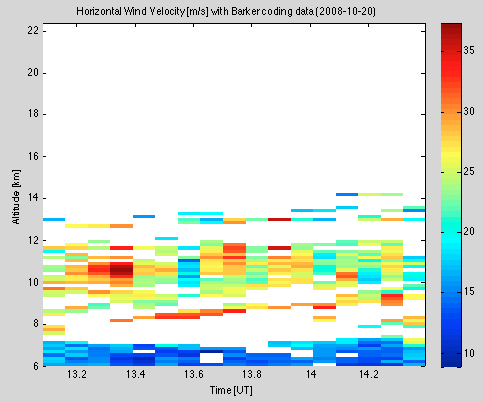
\includegraphics[width=8cm]{Figures/wind_vel_barker.png}
\caption{Horizontal wind velocity with Barker coding data.}
\label{fig:wind_vel_barker}
\end{minipage}
\end{figure}

\begin{figure}[htb]
\begin{minipage}[t]{0.5\linewidth}
\centering
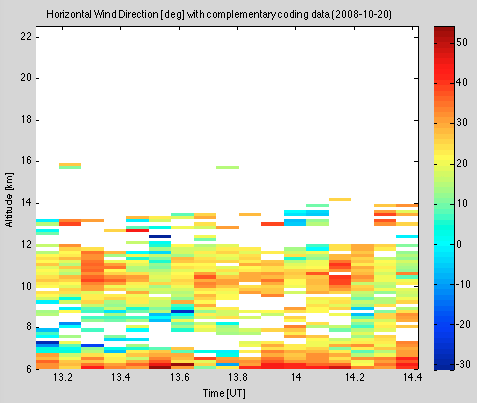
\includegraphics[width=8cm]{Figures/wind_dir_complementary.png}
\caption{Horizontal wind direction with complementary coding data.}
\label{fig:wind_dir_complementary}
\end{minipage}
\begin{minipage}[t]{0.5\linewidth}
\centering
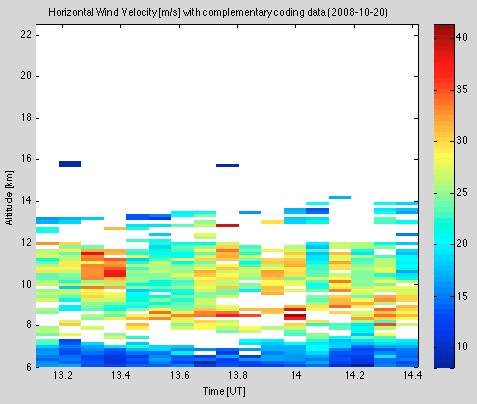
\includegraphics[width=8cm]{Figures/wind_vel_complementary.png}
\caption{Horizontal wind velocity with complementary coding data.}
\label{fig:wind_vel_complementary}
\end{minipage}
\end{figure}

\begin{figure}[htb]
\begin{minipage}[t]{0.5\linewidth}
\centering
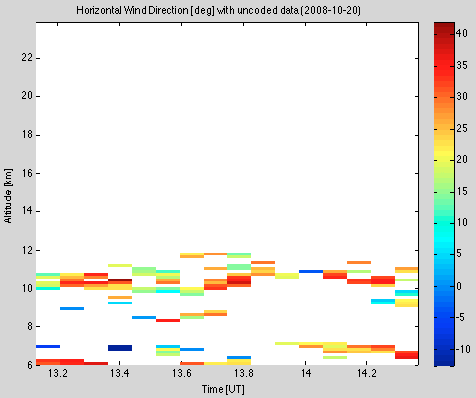
\includegraphics[width=8cm]{Figures/wind_dir_uncoded.png}
\caption{Horizontal wind direction with uncoded data.}
\label{fig:wind_dir_uncoded}
\end{minipage}
\begin{minipage}[t]{0.5\linewidth}
\centering
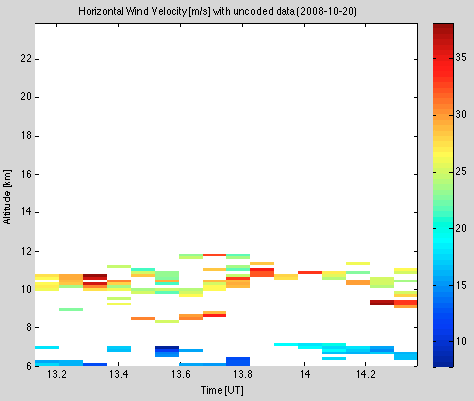
\includegraphics[width=8cm]{Figures/wind_vel_uncoded.png}
\caption{Horizontal wind velocity with uncoded data.}
\label{fig:wind_vel_uncoded}
\end{minipage}
\end{figure}


%----------------------------------------------------------------------------------------
%	SECTION 4. REFERENCES
%----------------------------------------------------------------------------------------

\begin{thebibliography}{9}

\bibitem{Enmark:2012a2}
Enmark, A.  (2012).
\newblock {\em Assignment 2. Pulse Modulation Techniques}.
\newblock Lule\aa \ University of Technology, Kiruna, Sweden.

\end{thebibliography}

%----------------------------------------------------------------------------------------
%	SECTION 5. Appendix 2A
%----------------------------------------------------------------------------------------

\section{Appendix 2A. Matlab code of Part 2A}

\subsection{Part2A.m}
\lstinputlisting{Part2A.m}

\subsection{plotSNR.m}
\lstinputlisting{plotSNR.m}

%----------------------------------------------------------------------------------------
%	SECTION 6. Appendix 2B
%----------------------------------------------------------------------------------------

\section{Appendix 2B. Matlab code of Part 2B}

\subsection{Part2B.m}
\lstinputlisting{Part2B.m}

\subsection{plotWind.m}
\lstinputlisting{plotWind.m}

\subsection{hypotenuse.m}
\lstinputlisting{hypotenuse.m}

\subsection{radToDeg.m}
\lstinputlisting{radToDeg.m}

%----------------------------------------------------------------------------------------
%	SECTION 7. Confirmation
%----------------------------------------------------------------------------------------

\section{Acknowledgements}


\end{document}